
\chapter{Methodik}

In diesem Kapitel wird die allgemeine Methodik der vorliegenden Arbeit beschrieben.

\section{3D Gaussian Splatting}

Zunächst wird untersucht, ob die neuartige Methode Gaussian Splatting für die 3D-Szenenrekonstruktion im Neural Space Time Lab (NSTL) geeignet ist.
Dazu wird COLMAP als Standardmethode zur Initialisierung mit einer Kalibrierung der Kameraparameter mithilfe von OpenCV verglichen, um Unterschiede in Genauigkeit und Leistung aufzuzeigen.

\subsection{Datensatzvorbereitung}
\label{sec:Datensatzvorbereitung}
Die Datensätze müssen in ein geeignetes Format gebracht werden, um sie im System nutzbar zu machen.

\subsubsection{COLMAP}

Die Bilder werden für COLMAP mithilfe eines bereitgestellten Skripts vorverarbeitet, das Feature Matching durchführt und eine grobe Punktwolke für die Initialisierung der 3D-Gaussians erstellt. 
Anschließend werden die Bilder mit den geschätzten Kameraparametern auf eine optimale Pinhole-Kamera entzerrt.

\subsubsection{OpenCV}
Die Vorverarbeitung mit OpenCV ist aufgrund der manuellen Kalibrierung zeitaufwendiger. 
Die Kameras im NSTL wurden zuvor intrinsisch und extrinsisch kalibriert, und diese Kalibrierung wird nun zur Entzerrung der Bilder verwendet.

\subsubsection{Entzerrung}
Gaussian Splatting setzt voraus, dass der Hauptpunkt der Kameramatrix im Bildzentrum liegt. Die Kameras im NSTL weisen jedoch einen versetzten Hauptpunkt von bis zu 40 Pixeln auf, was zu Projektionsfehlern führen kann. Mithilfe der OpenCV-Funktion newOptimalCameraMatrix mit alpha=0 werden die Bilder entzerrt, sodass der Hauptpunkt zentriert wird, ohne ungültige Bildbereiche hinzuzufügen. Dabei gehen jedoch an den Rändern Teile der Bildinformationen verloren. Diese Korrektur ist entscheidend, um die Konsistenz in Multi-View-Systemen zu gewährleisten und die räumliche Kohärenz in Gaussian Splatting zu erhalten. Die entzerrten Bilder und aktualisierten Kameramatrizen werden für das Training gespeichert.

\subsection{Camera Metadata in Json Format}
Nach der Vorverarbeitung werden die Kamerametadaten in einer transforms.json-Datei gespeichert, die Gaussian Splatting zum Laden der Daten nutzt. Diese JSON-Struktur enthält für jeden Frame den Dateipfad des Bildes, eine 4x4-Transformationsmatrix aus der extrinsischen Kalibrierung (Welt-zu-Kamera-Transformation) sowie die im vorherigen Schritt aktualisierte 3x3-Kameramatrix.

\subsection{Trainingsansätze}


Zur Validierung der Methode des 3D Gaussian Splatting wurde zunächst die Szene \textit{bicycle} aus dem Mip-NeRF 360 Datensatz \cite{barron2021mip} verwendet, um die im Referenzpaper \cite{kerbl3Dgaussians} angegebenen Ergebnisse zu reproduzieren. Diese Szene wurde gewählt, da sie im Paper ausführlich beschrieben ist und eine Vergleichbarkeit der Metriken wie SSIM, PSNR und LPIPS ermöglicht. Das Training wurde mit den Standardparametern der Methode durchgeführt und die Ergebnisse des Trainings nach 30.000 Iterationen miteinander verglichen.
Die Ergebnisse zeigten eine hohe Übereinstimmung mit den Literaturwerten, wie im Ergebnis-Teil (Kapitel~\ref{chap:Ergebnisse}) detailliert beschrieben.

Nach erfolgreicher Validierung wurden Experimente mit einem neu aufgenommenen Datensatz aus dem Neural Space Time Lab (NSTL) durchgeführt. Dieser Datensatz wurde zweifach vorbereitet.
Zum einen mit der COLMAP-Methode und zum anderen mit OpenCV, um die Auswirkungen der unterschiedlichen Kalibrierungsansätze auf die Rekonstruktionsqualität zu vergleichen. 
Die Ergebnisse zeigten, dass die Rekonstruktionen in der Region of Interest (ROI) im Zentrum des Raumes nahezu identisch waren, mit nur geringfügigen Unterschieden in den Metriken (siehe Kapitel~\ref{chap:Ergebnisse}).

Die Kalibrierung mit OpenCV erwies sich jedoch als vorteilhafter für die Anwendung im NSTL. 
Für die Kalibrierung mit OpenCV nutzt das Institut eine deterministische Kalibrierung mithilfe eines Charucoboards zur Bestimmung der intrinsischen und extrinsischen Kameraparameter.


Dadurch wird ein Koordinatensystem in realen Maßeinheiten (in diesem Fall Meter) definiert, das eine präzise und für den Menschen nachvollziehbare Zuordnung räumlicher Positionen ermöglicht.
Diese Eigenschaft ist besonders wichtig für die Integration mit anderen Systemen im Neural Space Time Lab (NSTL), wo exakte räumliche Beziehungen für die Multikameradaten erforderlich sind. 
Im Gegensatz dazu verwendet COLMAP eine Struktur-aus-Bewegung (SfM)-Methode, die Kameraparameter und ein synthetisches Koordinatensystem durch Feature Matching und iterative Optimierung schätzt. 
Dieses Koordinatensystem ist nicht in realen Maßeinheiten definiert und erfordert eine nachträgliche Skalierung, die zusätzliche Unsicherheiten in die Rekonstruktion einführt. 
Die deterministische Kalibrierung mit OpenCV und dem Charucoboard gewährleistet eine höhere Genauigkeit und Konsistenz über verschiedene Szenen hinweg, da sie keine szenenspezifischen Abhängigkeiten der Kameraparameter aufweist. 

Obwohl COLMAP in vielen 3D-Rekonstruktionsanwendungen qualitativ hochwertigere Ergebnisse liefern kann, wird OpenCV im NSTL-Kontext bevorzugt. Dies liegt an der robusten und reproduzierbaren Kalibrierung, die eine direkte Übertragbarkeit der Kameraparameter auf verschiedene Szenen ermöglicht und die Notwendigkeit nachträglicher Anpassungen minimiert.
Daher stellt OpenCV eine stabilere und für die Anforderungen des NSTL besser geeignete Grundlage für die weitere Untersuchung von 3D- und 4D-Gaussian-Splatting-Anwendungen dar.



\section{Darstellung von neuen Ansichten und Tiefenbildern}
\label{sec:new_views_depth}

Ein wesentlicher Vorteil des 3D Gaussian Splatting besteht darin, dass die zugrunde liegende Repräsentation nicht an die diskreten Kamerapositionen der Trainingsdaten gebunden ist. 
Da die Szene als kontinuierliche Punktwolke in Form anisotroper Gaussians modelliert wird, können beliebige neue Kamerapositionen definiert und für die Erzeugung von Ansichten genutzt werden. 
Dies ermöglicht es, auch Perspektiven zu rendern, die im Trainingsprozess nicht enthalten waren. 
Abbildung~\ref{fig:cam_setup} zeigt hierzu exemplarisch die Positionen der Trainingskameras, die die Grundlage für die Optimierung des Modells bilden. 
Darüber hinaus lassen sich neue Kamerapfade definieren, um Ansichten aus frei gewählten Positionen zu generieren. 
Dies eröffnet den Zugang zu einer Vielzahl zusätzlicher Darstellungen, die insbesondere für Visualisierungen und qualitative Analysen von Vorteil sind. 

Neben Farbbildern können durch den Rasterisierungsprozess auch Tiefenkarten erzeugt werden. 
Diese stellen die geometrische Struktur der rekonstruierten Szene dar und liefern damit eine zusätzliche Modalität zur Analyse der Rekonstruktion. 
Tiefenbilder sind vor allem für Anwendungen in der Robotik oder für die Integration mit weiteren Sensorsystemen von Bedeutung, da sie die Lageinformation einzelner Strukturen im Raum unmittelbar erfassbar machen. 
Ein Beispiel für eine generierte Tiefenkarte ist in Abbildung~\ref{fig:depth_example} dargestellt.

Die detaillierte Auswertung der erzeugten Bilder erfolgt im Ergebnisteil dieser Arbeit. 
Zusätzliche Darstellungen von Ansichten außerhalb der Trainingskameras sowie von Tiefenkarten sind im Anhang enthalten, um die Vielseitigkeit der Methode zu illustrieren, ohne den Ergebnisabschnitt durch eine Vielzahl visueller Beispiele zu überfrachten.

% \begin{figure}[h]
%     \centering
%     \includegraphics[width=0.7\linewidth]{bilder/methods/camera_setup.png}
%     \caption{Schematische Darstellung der verwendeten Trainingskameras: Die kontinuierliche Repräsentation der Szene erlaubt es, beliebige zusätzliche Ansichten durch neue Kamerapositionen zu erzeugen.}
%     \label{fig:cam_setup}
% \end{figure}

% \begin{figure}[h]
%     \centering
%     \includegraphics[width=0.7\linewidth]{bilder/methods/depth_example.png}
%     \caption{Beispiel einer aus 3D Gaussian Splatting generierten Tiefenkarte: Neben Farbbildern lassen sich auch geometrische Informationen in Form von Tiefenbildern extrahieren.}
%     \label{fig:depth_example}
% \end{figure}
















\section{4D Gaussian Splatting}

Im vorherigen Abschnitt wurde die Methode des 3D Gaussian Splatting vorgestellt und ihre Anwendbarkeit für die Rekonstruktion statischer Szenen im Neural Space Time Lab (NSTL) validiert.
Das NSTL ermöglicht jedoch auch die Aufnahme zeitsynchroner Daten, wodurch die zeitliche Komponente in die Rekonstruktion einbezogen werden kann.
Für die Modellierung dynamischer Szenen ist daher eine Erweiterung auf 4D Gaussian Splatting erforderlich, das die Bewegung und Veränderungen über die Zeit hinweg berücksichtigt. Die Vorverarbeitung der Daten bleibt dabei identisch zu 3D Gaussian Splatting.
Die Bilder werden entzerrt, und die Kamerametadaten werden im JSON-Format strukturiert. Zusätzlich werden nun Zeitstempel zu den Kameradaten hinzugefügt, um die zeitlichen Abstände zwischen den Bildern eindeutig zu definieren. 
Diese Zeitstempel bilden die Grundlage, um die Multikameradaten des NSTL in eine kohärente, zeitliche Rekonstruktion zu überführen.
Da verschiedene Ansätze zur Modellierung dynamischer Szenen existieren, wurde eine Methode gesucht, die sowohl die räumliche als auch die zeitliche Kohärenz effizient abbildet. 


\section{4DGS by Wang et al.}

Die Methode von Wang et al. \cite{yang20244dgs} wurde aufgrund ihrer überlegenen Renderinggeschwindigkeit und Rekonstruktionsqualität ausgewählt. Im Vergleich zu anderen Ansätzen, wie etwa Wu et al. \cite{wu20244d}, zeigte sie in der Literatur bessere Ergebnisse bei gängigen Metriken wie PSNR und SSIM sowie eine bis zu dreifache Renderinggeschwindigkeit. Diese Eigenschaften machen sie besonders geeignet für die Erzeugung neuer Daten aus dynamischen Szenen im Neural Space Time Lab (NSTL). Im Folgenden werden die Trainingsansätze, Verbesserungsansätze und ein speziell für den NSTL entwickelter Ansatz für das Training mit festem Hintergrund vorgestellt.

\subsection{Validierung der Methode}
Zur Validierung der Methode von Wang et al. wurde ein ähnlicher Ansatz wie bei 3D Gaussian Splatting verfolgt, um die Reproduzierbarkeit der im Referenzpaper \cite{yang20244dgs} angegebenen Ergebnisse zu überprüfen. Dazu wurden zwei Testdatensätze verwendet: eine synthetische Szene aus dem D-NeRF-Datensatz \cite{pumarola2020dnerf}, bestehend aus 100 Frames mit einer dynamischen Figur, und eine Szene aus dem Plenoptic-Datensatz \cite{li2022neural}, die 50 Frames mit komplexen Bewegungen umfasst.
Beide Datensätze wurden mit den Standardparametern der Methode trainiert, welche in den zugehörigen yaml-Files abgelegt werden. 
Die Ergebnisse zeigten eine hohe Übereinstimmung mit den Literaturwerten, wie im Ergebnis-Teil (Kapitel~\ref{chap:Ergebnisse}) detailliert beschrieben.


\subsection{Datensätze aus dem NSTL}

Anschließend wurde die Methode auf einen neu aufgenommenen Datensatz angewendet.
Der erste Datensatz umfasste 200 Frames, welche mit 30 FPS aufgenommen wurden und somit eine Zeitspanne von 6.6 Sekunden abbildet.
Die Szene zeigt eine Person, die die Arme auf und ab bewegt und sich währenddessen im Kreis dreht. 
Zuerst wurden Experimente zur Analyse der Qualität mit verschiedener Anzahl an Gaussians durchgeführt. 
Dabei wurde schnell ersichtlich, dass die Qualität stark von der Anzahl an Gaussians abhängig ist.
In \ref{sec:results_4dgs} sind die Ergebnisse dazu dargestellt.

Leider konnte aufgrund von Hardwarebegrenzungen die Anzahl der Gaussians nicht weiter erhöht werden, da sonst der Speicher überläuft und das Training beendet.
Deshalb wurde die Länge der Szene auf ein Viertel gekürzt und nur noch die ersten 50 Frames und somit 1.6 Sekunden betrachtet.
Dies reduziert die Komplexität der Szene weiter, da deutlich weniger Zeitschritte modelliert werden müssen und somit in wichtigen, sich schnell bewegenden Bereichen wie den Händen der Person mehr Gaussians genutzt werden können als zuvor mit der kompletten Szene.



\subsection{Analyse der temporalen Redundanz}

Das Paper von Yuan et al.~\cite{yuan20251000fps4dgaussian} zeigte, dass die hohen Speicherkosten der Methode von Wang et al.~\cite{wang20234dgs} maßgeblich durch kurzlebige Gaussians verursacht werden, selbst in Szenen mit überwiegend statischem Hintergrund. 
Solche kurzlebigen Gaussians tragen oft nur für wenige Frames zur Bildinformation bei und verschwinden anschließend wieder, wodurch redundante Daten entstehen, die den Speicherverbrauch erhöhen, ohne einen nachhaltigen Beitrag zur Szenenrepräsentation zu leisten.  

\subsubsection{Empirische Analyse}  
Zuerst wurde untersucht, ob die Aussagen aus dem Paper auch in den Modellen aus dem NSTL-Datensatz auftreten.
Zur Untersuchung wurde das finale Modell mit den 50 Frames des NSTL-Datensatzes analysiert.  
In Abb.~\ref{fig:gaussians_percentage} wird der Wert der Kovarianz dargestellt, der dafür verantwortlich ist, wie lange ein Gaussian innerhalb einer Szene aktiv ist und somit zum gegebenen Zeitschritt beiträgt.
Dabei ist klar ersichtlich, dass der Großteil der Gaussians einen sehr geringen Wert für die zeitliche Kovarianz aufweist und somit nur in einzelnen aufeinanderfolgenden Zeitschritten aktiv ist. 
Abb.~\ref{fig:gaussians_active} zeigt, dass das aktive Set an Gaussians nur etwa 20\% der Gesamtheit ausmacht und somit 80\% der Gaussians nicht zum aktuellen Zeitschritt beitragen.

Da die Metriken die gleichen Charakteristika zeigen wie im Paper beschrieben, wurde der Spatial-Temporal Score aus dem Paper nachimplementiert, um ihn nutzbar zu machen und somit das Modell effizienter zu gestalten.
Dadurch stehen mehr Rechenressourcen für noch unterrekonstruierte Bereiche der Szene zur Verfügung.
Da keine offizielle Implementierung vorhanden ist, wurde sich an früheren Arbeiten orientiert.

\subsubsection{Spatial Score}  
Um den visuellen Beitrag eines Gaussians $g_i$ zu einem gegebenen Zeitpunkt zu messen, wurde der Spatial Score entwickelt.
Der Spatial Score aggregiert den Strahlenbeitrag eines Gaussians über alle Strahlen $r$ und über alle Eingabebilder zu einem Zeitpunkt:  
\[
S_i^S = \sum_{k=1}^{NHW} \alpha_i \prod_{j=1}^{i-1} (1 - \alpha_j)
\]
wobei $\alpha_i \prod_{j=1}^{i-1} (1 - \alpha_j)$ den Beitrag des $i$-ten Gaussians zur finalen Farbe gemäß Alpha-Komposition widerspiegelt.
Bei der Implementierung wurde sich stark an \emph{lightgaussian} orientiert.
\emph{Lightgaussian} implementiert den Spatial Score für 3D Gaussian Splatting im tile-based Rasterizer, um eine effiziente Berechnung des Spatial Scores zu ermöglichen.
Die Implementierung im Rasterizer konnte somit fast vollständig übernommen und lediglich für den 4D-Fall erweitert werden.

\subsubsection{Temporal Score}  
Entscheidend für die Bewertung der Kurzlebigkeit der Gaussians ist der Temporal Score.
Er gibt Gaussians, die nur kurze Zeit zur Szenenrepräsentation beitragen, einen entsprechend schlechten Score.
Die zeitliche Stabilität wird durch die zweite Ableitung der temporalen Opazitätsfunktion $p_i(t)$ erfasst:
\[
p_i^{(2)}(t) = \left( \frac{(t - \mu_t)^2}{\Sigma_t^2} - \frac{1}{\Sigma_t} \right) p_i(t)
\]
Zur Normierung in das Intervall $(0, 1)$ wird die $\tanh$-Funktion angewendet, woraus der \emph{Temporal Variation Score} $S_i^{TV}$ resultiert:
\[
S_i^{TV} = \sum_{t=0}^{T}  \frac{1}{\left( 0.5 \cdot   \tanh(\lvert p_i^{(2)}(t) \rvert) + 0.5 \right)}
\]
Zusätzlich wird das Volumen des 4D-Gaussians berücksichtigt und normalisiert:
\[
\gamma(S_{4D}) = \text{Norm}(V(S^{4D}))
\]
Der finale \emph{Temporal Score} ergibt sich zu:
\[
S_i^T = S_i^{TV} \cdot \gamma(S_i^{4D})
\]

\subsubsection{Spatial-Temporal Score}  

Der \emph{Spatial-Temporal Variation Score} $S_i$ kombiniert beide Metriken:
\[
S_i = \sum_{t=0}^{T} S_i^T \cdot S_i^S
\]
Dadurch lassen sich Gaussians identifizieren, die sowohl einen hohen visuellen Beitrag als auch eine hohe zeitliche Persistenz aufweisen.

\subsubsection{Training}
Nach der Implementierung konnte der neue Spatial-Temporal Score während des Trainings verwendet werden. 
Zunächst ging es darum zu validieren, wie das Pruning der Gaussians die Ergebnisse der Rekonstruktion beeinflusst.
Dazu wurde zunächst, wie im Paper beschrieben, das Pruning erst nach der vollständigen Densification durchgeführt, wobei Gaussians mit einem schlechten Spatial-Temporal Score entfernt wurden.
Anschließend wurde ein Training gestartet, bei dem das Pruning bereits während der Densification stattfand.
Dies sollte das Ziel haben, Gaussians mit einem schlechten Score frühzeitig zu entfernen und durch neue mit einem besseren Score zu ersetzen.
Die Bewertung der Effektivität dieser Verfahren und deren Einfluss auf Speicherverbrauch und visuelle Qualität erfolgt in Abschnitt~\ref{pruning_results}.


\subsubsection{Eigener Tennis-Volley-Datensatz}

Um den Einfluss redundanter Hintergrund-Gaussians auf Speicherverbrauch und Bildqualität besser zu kontrollieren, wurde ein zusätzlicher Datensatz aufgenommen. 
Dabei wurde der Aufnahmeort gezielt vereinfacht: Der Raum wurde aufgeräumt, der Vorhang geschlossen und auf weitere Personen verzichtet. 
Dadurch sollte vermieden werden, dass Gaussians auf Bereiche außerhalb der eigentlichen Szene verteilt werden und somit unnötig Speicher beanspruchen.

Das Training erfolgte mit denselben Parametern und Evaluationsmetriken wie in den vorherigen Experimenten, sodass die Ergebnisse konsistent eingeordnet werden können. 
Besonderes Augenmerk liegt hier auf der Frage, ob durch den bereinigten Hintergrund eine geringere Anzahl an Gaussians erforderlich ist, um die Szene zu modellieren.





\subsection{Training mit festem Hintergrund}




Die Experimente mit dem Tennis-Volley-Datensatz verdeutlichten, dass bereits durch eine gezielte Bereinigung der Szene die Anzahl der benötigten Gaussians deutlich reduziert werden kann. 
Dies führte nicht nur zu geringerem Speicherverbrauch, sondern zugleich zu einer spürbar höheren Bildqualität. 
Allerdings war das Training weiterhin auf kurze Sequenzen von maximal 50 Frames beschränkt, da ansonsten die VRAM-Kapazität überschritten wird. 
Dies zeigt, dass trotz optimierter Datensatzgestaltung die Speichereffizienz weiterhin ein limitierender Faktor bleibt. 

Vor diesem Hintergrund entstand der Ansatz, die spezifischen Eigenschaften des NSTL-Setups algorithmisch auszunutzen.
Die Kameras sind fest installiert und liefern vor Beginn der Bewegungssequenz jeweils ein Bild des leeren Raums. 
Somit steht für jede Kamera sowohl ein Referenzbild der statischen Szene als auch die eigentliche Bewegungssequenz zur Verfügung. 
Ziel ist es, den statischen Hintergrund direkt in das Training einzubinden, sodass Gaussians gezielt auf die dynamischen Inhalte fokussiert werden können. 
Durch diese Einbettung können weniger Gaussians für den Hintergrund verwendet werden, der VRAM wird effizienter genutzt, und die Modellierung relevanter Bewegungen kann auch bei längeren Sequenzen präziser erfolgen. 

Der Ansatz greift in den Rasterisierungsprozess ein. 
Während der Standard-Rasterisierung werden die einzelnen Gaussians auf die Bildebene projiziert und ihre Farbinformationen unter Berücksichtigung der Transmittanz akkumuliert. 
Bleibt die akkumulierte Transmittanz für einen Pixel kleiner als eins, wird im Standardverfahren die verbleibende Fläche mit einer festen Hintergrundfarbe gefüllt. 
Üblicherweise wird hierfür Schwarz verwendet.

In der modifizierten Variante wird dieser Schritt durch eine adaptive Hintergrundeinbettung ersetzt. 
Statt einer einheitlichen Farbe wird für jeden Pixel die Farbinformation aus dem zuvor aufgenommenen Referenzbild der entsprechenden Kamera eingefügt. 
Beim Laden der Daten wird dazu ebenfalls das entsprechende Hintergrundbild der Kamera übergeben.
Pixel, die im dynamischen Bild vollständig durch statische Geometrie erklärt werden, müssen nicht durch Gaussians abgedeckt werden, da ihre Farbwerte bereits exakt durch das Referenzbild repräsentiert werden. 

Gaussians werden primär in jenen Regionen platziert und optimiert, in denen Abweichungen zwischen der aktuellen Szene und dem Referenzbild bestehen. 
Dies betrifft insbesondere bewegte Objekte sowie deren Interaktionen mit der Umgebung, beispielsweise Schatten oder Spiegelungen. 
Konzeptionell entspricht dies der Berechnung eines Differenzbildes, bei dem ausschließlich die Veränderungen explizit modelliert werden.

Die Implementierung erfordert eine Erweiterung des Rasterizers um eine Hintergrund-Lookup-Funktion, die für jede Kamera und jeden Pixel den entsprechenden Wert aus dem Referenzbild abrufen kann. 
Zum Testen wurde zuerst zufällige Hintergrundbilder während eines normalen Rendering-Prozesses eingefügt.
Die Ergebnisse hierzu sind in Abschnitt \ref{sec:zufälligeHintergründe} dargestellt.

Durch die Auslagerung des statischen Szenenanteils in ein vorab aufgenommenes Hintergrundbild reduziert sich die Anzahl der zu optimierenden Gaussians im statischen Bereich auf nahezu null. 
Dies verringert den Speicherverbrauch und ermöglicht es, mehr VRAM für die Modellierung dynamischer Inhalte zu verwenden. 
Die Analyse der Effektivität dieser Methode sowie ihr Einfluss auf die visuelle Qualität und den Speicherbedarf werden in Kapitel~\ref{chap:Ergebnisse} beschrieben.









\section{4D Gaussians}

Trotz der hohen Rekonstruktionsqualität des Ansatzes von Wang et al. zeigen sich  wesentliche praktische Einschränkungen.
Insbesondere die Kombination aus hohem Speicherbedarf und fehlender Objektzuordnung erschwert weiterführende Aufgaben wie Segmentierung und Editing erheblich. Um diese Limitierungen zu adressieren, wurde die Methode von Wu et al. evaluiert, die anstelle expliziter Gaussians pro Frame Transformationen über ein MLP modelliert. Dieser Ansatz versprach eine kompaktere Darstellung und potenziell eine leichtere Integration in objektbezogene Anwendungen.
 
\subsection{Trainingsansätze}

Die Experimente mit Wu et al. zeigten jedoch, dass die Methode die komplexen Bewegungen im Multiview-Datensatz des NSTL nicht adäquat abbilden konnte. Die Rekonstruktionen waren verschwommen, insbesondere bei sich schnell bewegenden Objekten.
Aufgrund dieser Schwächen wurde eine weitere Methode evaluiert, die besser auf die
Anforderungen des NSTL abgestimmt ist.




\section{Dynamic 3D Gaussians}
\label{sec:method_dynamic3d}

Die Methode der Dynamic 3D Gaussians (vgl. Abschnitt~\ref{sec:sota_dynamic3d}) bietet durch die zeitliche Verschiebung und Wiederverwendung einer festen Menge an Gaussians die Möglichkeit, Speicherbedarf zu reduzieren und gleichzeitig eine objektzentrierte Repräsentation zu erzeugen. 
Im Folgenden wird beschrieben, wie diese Methode im Kontext des NSTL umgesetzt und angepasst wurde. 
Dazu werden zunächst die Datensätze und deren Vorbereitung vorgestellt, bevor anschließend die Implementationsdetails sowie verschiedene Trainingsvarianten diskutiert werden. 


\subsection{Validierung der Methode}

Analog zu den vorherigen Verfahren wurde auch Dynamic 3D Gaussians zunächst anhand einer Szene überprüft, für die in der Originalarbeit bereits Vergleichsergebnisse veröffentlicht wurden.
Dazu wurde die Szene Tennis aus dem Panoptic Sports Dataset gewählt, die von den Autoren einschließlich des erforderlichen Preprocessings bereitgestellt wird.
Durch diesen direkten Bezug lassen sich die im Rahmen dieser Arbeit erzielten Resultate konsistent mit den publizierten Referenzwerten vergleichen und die Implementierung verlässlich validieren.


\subsection{Datensatzvorbereitung}

Nachdem die Reproduzierbarkeit der Referenzergebnisse bestätigt werden konnte, wurde der Volley-Datensatz für die Anwendung von Dynamic 3D Gaussians vorbereitet. 
Der Datenaufbau unterscheidet sich nur geringfügig von den zuvor verwendeten Verfahren.
Es werden weiterhin RGB-Bilder sowie die zugehörigen intrinsischen und extrinsischen Kameramatrizen benötigt.
Zusätzlich werden für die vorliegende Methode Segmentierungen des bewegten Objekts (der Person inklusive Schläger) eingesetzt.

Zur Erzeugung dieser Segmentierungen wurden die Tiefenbilder verwendet, welche mithilfe des finalen Modells aus dem Training mit festem Hintergrund gerendert wurden. 
Dieses Vorgehen hat den Vorteil, dass in den gerenderten Tiefenaufnahmen überwiegend die Person und der Schläger sichtbar ist, wodurch sich eine robuste Trennung zwischen dynamischem Vordergrund und statischem Hintergrund erzielen lässt. 
Aus den Tiefenkarten wurde anschließend durch Schwellenwertbildung eine erste Binärmaske gewonnen ( Schwellwert $\tau \approx 0.7$ ). 
Zur Schließung kleiner Löcher in der Maske — insbesondere in den feinen Strukturen des Schlägers — wurde ein morphologisches Closing angewendet.

Diese Nachverarbeitung reduziert viele Lücken in der Schlägermaske, hat aber auch Nebeneffekte.
Vereinzelte Regionen, etwa Zwischenräume zwischen den Armen, wurden ebenfalls geschlossen, sodass die Maske an einigen Stellen leicht übersegmentiert ist. 
Abbildung~\ref{fig:Segmentation_D3DGS} zeigt oben links ein exemplarisches RGB-Bild und rechts die dazugehörige Tiefenkarte; darunter ist die resultierende Binärmaske nach Schwellenwertbildung und Morphologie dargestellt. 

Die weiterverarbeiteten Daten wurden im gleichen Format abgespeichert wie in Abschnitt~\ref{sec:Datensatzvorbereitung} beschrieben, sodass die Trainingspipeline unverändert weiterverwendet werden konnte.

% \begin{figure}[htbp]
%     \centering
%     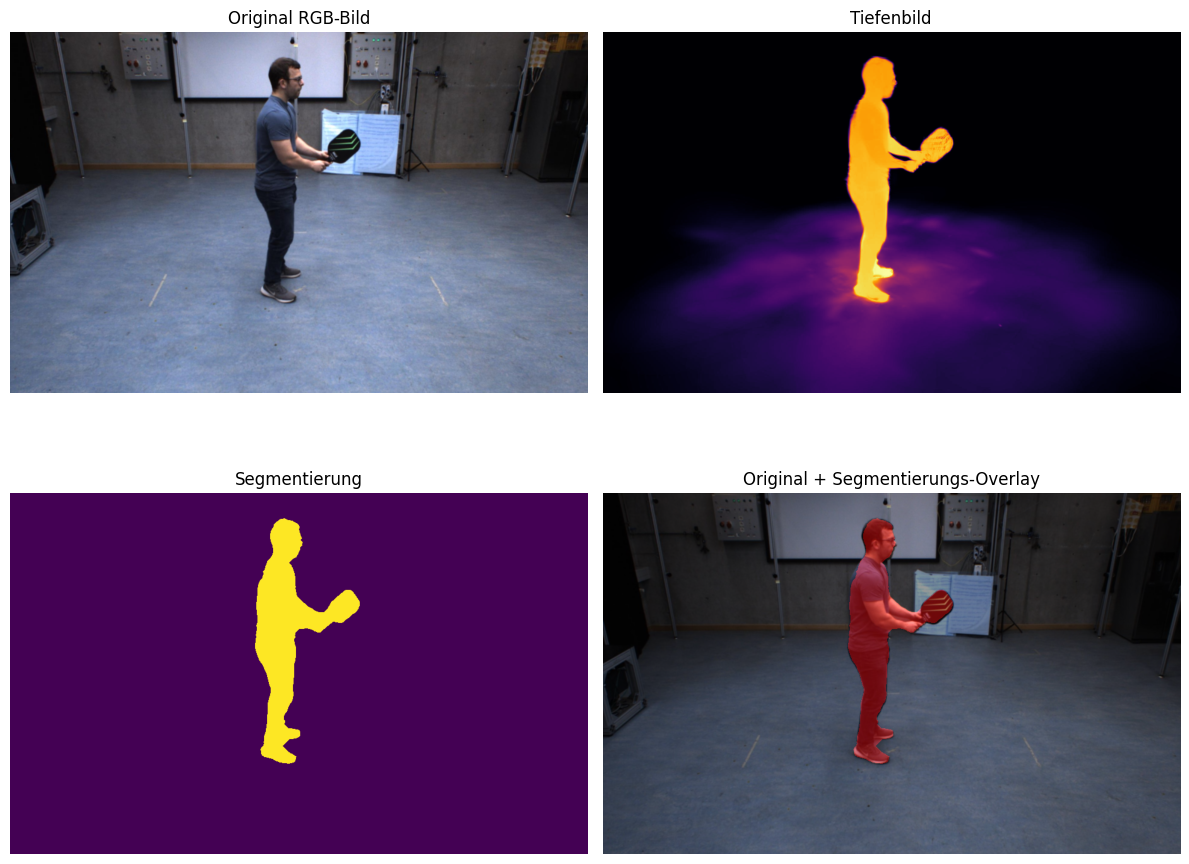
\includegraphics[width=1\linewidth]{bilder/Results/D3DGS/visualization_8.png}
%     \caption{Beispiel für die Maskenerzeugung: oben links Ground-Truth RGB, oben rechts gerenderte Tiefenkarte; unten die aus der Tiefenkarte abgeleitete Binärmaske nach Schwellenwertbildung und morphologischem Closing.}
%     \label{fig:Segmentation_D3DGS}
% \end{figure}


\subsection{Trainingsansätze}

Zunächst wurde das Modell mit dem im vorherigen Abschnitt beschriebenen, vorbereiteten Datensatz trainiert. 
In einem ersten Schritt kamen alle in der Originalimplementierung vorgesehenen Parameter und Verlustterme unverändert zum Einsatz. 
Dabei zeigte sich jedoch, dass insbesondere die zusätzlichen Kamera-Parameter \texttt{cam\_c} und \texttt{cam\_m}, welche Helligkeit und Kontrast der gerenderten Bilder steuern, die Farbdarstellung im NSTL stark verfälschten. 
Um eine stabilere Trainingsdynamik und konsistentere Farbtreue zu gewährleisten, wurden diese Parameter aus der Optimierung entfernt und stattdessen fixiert.  

Ein weiterer Anpassungsschritt betrifft den in der Originalarbeit enthaltenen sogenannten \emph{Floor-Loss}. 
Dieser bestraft Punkte, die unterhalb der Ebene $y=0$ liegen, und dient damit der Stabilisierung in Szenen mit bekanntem Bodenverlauf. 
Im NSTL verläuft die $y=0$-Ebene jedoch schräg durch den Raum, sodass der Verlust hier ungewollt auch relevante Vordergrundstrukturen bestraft hätte. 
Der Floor-Loss wurde daher vollständig deaktiviert. 
% Ein Plot zur Visualisierung dieses Problems befindet sich in Anhang~\ref{sec:appendix_floorloss}.  

% Die beschriebenen Anpassungen führten zu den bislang stabilsten Trainingsläufen. 
% Weitere Varianten – etwa eine Einschränkung des L1-Anteils im Bildverlust auf relevante Regionen – wurden konzeptionell vorbereitet, konnten im Rahmen dieser Arbeit jedoch nicht mehr umfassend untersucht werden.



% \subsection{Implementationsdetails}

% Welche Basis du übernommen hast (z. B. offizielle Implementierung von Luiten).

% Welche Parameter im Training angepasst wurden (Batchgrößen, Speichergrenzen, VRAM-Limit bei 50 Frames).

% Nutzung des festen Hintergrunds in Kombination mit Dynamic 3DGS.

% \subsection{Trainingsvarianten}

% Hier listest du nur deine Iterationen und Modifikationen, ohne das ganze Grundprinzip zu wiederholen:

% Entfernen von \texttt{cam_c} und \texttt{cam_m}.

% Entfernen des Floor Loss aufgrund schiefem Koordinatensystem.

% Unterschiedliche Initialisierungen: zufällige Punktewolke vs. PLY-Loader vs. mittlere Gaussians.

% Varianten mit/ohne Segmentierung.

% Nur mittlere Gaussians dynamisch, andere statisch.

% Daraus kannst du zwei Unterkapitel machen:

% Ablationsstudien (kurze Darstellung aller Varianten, ggf. Abbildung oder Tabelle mit qualitativen Beispielen, Hauptteil + Rest in Anhang).

% Optimale Konfiguration (die Variante, die im Rest der Arbeit verwendet wird).

% \subsection{Diskussion der Limitationen}

% Speichergrenze bei 50 Frames.

% Qualitäts-Tradeoff bei schnellen Bewegungen.

% Probleme mit Metriken, da Hintergrund nicht mitgerendert wird.




